\documentclass[12pt,letterpaper, onecolumn]{exam}
\usepackage{amsmath}
\usepackage{amssymb}
\usepackage{sidecap}
\usepackage{tabularx}
\usepackage{csquotes}
\usepackage{makecell}
\usepackage{hyperref}
\hypersetup{
    colorlinks=true,
    linkcolor=blue,
    filecolor=magenta,      
    urlcolor=black,
    pdftitle={Overleaf Example},
    pdfpagemode=FullScreen,
}
%\usepackage[left=0.5cm,right=0.5cm,top=0.5cm,bottom=0.5cm]{geometry}
\usepackage[usestackEOL]{stackengine}
%\setstacktabbedgap{1ex} 
\usepackage{tikz}
\usetikzlibrary{decorations.pathreplacing}
\usetikzlibrary{fadings}
\def\layersep{2.5cm}

\usepackage{enumitem}

%\usepackage[shortlabels]{enumitem}
%\usepackage{enumerate}
\usepackage[lmargin=71pt, tmargin=0.8in]{geometry}  %For centering solution box

% \chead{\hline} % Un-comment to draw line below header
\thispagestyle{empty}   %For removing header/footer from page 1

\usepackage{listings}
\usepackage{xcolor}

\definecolor{codegreen}{rgb}{0,0.6,0}
\definecolor{codegray}{rgb}{0.5,0.5,0.5}
\definecolor{codepurple}{rgb}{0.58,0,0.82}
\definecolor{backcolour}{rgb}{0.95,0.95,0.92}

\lstdefinestyle{mystyle}{
    backgroundcolor=\color{backcolour},   
    commentstyle=\color{codegreen},
    keywordstyle=\color{magenta},
    numberstyle=\tiny\color{codegray},
    stringstyle=\color{codepurple},
    basicstyle=\ttfamily\footnotesize,
    breakatwhitespace=false,         
    breaklines=true,                 
    captionpos=b,                    
    keepspaces=true,                 
    numbers=left,                    
    numbersep=5pt,                  
    showspaces=false,                
    showstringspaces=false,
    showtabs=false,                  
    tabsize=2
}

\lstset{style=mystyle}




\begin{document}



\newtheorem{theorem}{Theorem}[section]
\newtheorem{problem}{Problem}
\newtheorem{proposition}{Proposition}[section]
\newtheorem{lemma}{Lemma}[section]
\newtheorem{corollary}[theorem]{Corollary}
\newtheorem{example}{Example}[section]
\newtheorem{definition}[problem]{Definition}

\newcommand{\BEQA}{\begin{eqnarray}}
\newcommand{\EEQA}{\end{eqnarray}}
\newcommand{\define}{\stackrel{\triangle}{=}}
\bibliographystyle{IEEEtran}
\raggedbottom
\setlength{\parindent}{0pt}
\providecommand{\mbf}{\mathbf}
\providecommand{\norm}[1]{\lVert#1\rVert}
\providecommand{\pr}[1]{\ensuremath{\Pr\left(#1\right)}}
\providecommand{\qfunc}[1]{\ensuremath{Q\left(#1\right)}}
\providecommand{\sbrak}[1]{\ensuremath{{}\left[#1\right]}}
\providecommand{\lsbrak}[1]{\ensuremath{{}\left[#1\right.}}
\providecommand{\rsbrak}[1]{\ensuremath{{}\left.#1\right]}}
\providecommand{\brak}[1]{\ensuremath{\left(#1\right)}}
\providecommand{\lbrak}[1]{\ensuremath{\left(#1\right.}}
\providecommand{\rbrak}[1]{\ensuremath{\left.#1\right)}}
\providecommand{\cbrak}[1]{\ensuremath{\left\{#1\right\}}}
\providecommand{\lcbrak}[1]{\ensuremath{\left\{#1\right.}}
\providecommand{\rcbrak}[1]{\ensuremath{\left.#1\right\}}}
\let\vec\mathbf

\newlist{mydesc}{description}{1} % create a new list called mydesc, of type "description"
\setlist[mydesc]{
  align=left, % use the align-format defined above
  leftmargin=0pt, % indentation for all the lines
  labelindent=1em, % horizontal space before label
  labelsep=0pt
   % horizontal space after label -- set to zero because we add space via "leftwithbar"
}



\begingroup  
    \centering
    
    \LARGE Weekly Report 1-Logistic Regression\\[0.5em]
    \large \today\\[0.5em]
    \large Ganji Varshitha\par
    \large AI20BTECH11009\par
\endgroup
\rule{\textwidth}{0.4pt}
\pointsdroppedatright   %Self-explanatory
\printanswers
\newcommand\Solution{
  \textbf{Solution:}\\}
\newcommand{\myvec}[1]{\ensuremath{\begin{bmatrix}#1\end{bmatrix}}}
 %Replace "Ans:" with starting keyword in solution box

\subsection*{Introduction}
Logistic regression is a misnomer since it is a classification algorithm. Unlike linear regression which outputs continuous number values, logistic regression transforms its output using the logistic sigmoid function to return a probability value which can then be mapped to two or more discrete classes.
\subsection*{Algorithm}
We try to fit the data into a curved 'S' like graph unlike the straight line graph in linear regression. \\
The name of the algorithm comes from the function which is used to transform its output to return a probability value which can then be mapped to two or more discrete classes. \\

We assume functional form of $P(Y|X)$ and estimate parameters of $P(Y|X)$ directly from training data.\\

Let $p_y(x;w)$ be our estimate of $P(Y|X)$, where $\vec{w}$ is a vector of adjustable parameters. \\

\begin{align}
P(Y=1|X,\vec{w}) = {}&\frac{1}{1+\exp{(-\vec{w}^\top X)}}
\end{align}

In case of binary class problem, log odds of y or logit transformation of y is a linear function of x.\\Inverse of logit is the Logistic function which is sigmoid function for binary class problem.\\ We estimate $\vec{w}$ using maximum likelihood estimation.
\begin{align}
\vec{w} = {}& \arg \max_{\vec{w}} \sum_{l} \text{ln} P(y^l|\vec{x}^l,\vec{w})
\end{align}
This involves minimising negative likelihood which is convex.\\
We use gradient descent for the minimisation problem by updating the weights in the direction of gradient.

\subsection*{Key points}
\begin{itemize}
\item It does not assume on $P(X|Y)$ and learns the parameters that maximises the conditional probability $P(Y|X)$.
\item It is a discriminative model which draws boundaries in the data space and focusses on predicting the labels.
\item After predicting the probabilities of the output belong to a class, we need to map the probabilities to classes by using the decision threshold.
\item It is a linear classifier as the decision rule is hyperplane.
\item Softmax activation is used for multi class logistic regression.
\end{itemize}

\begin{figure}[!h]
\caption{Algorithm for binary class gradient descent(Logistic Regression)}
\centering
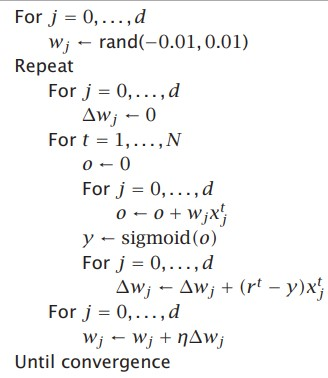
\includegraphics[width = 0.4\textwidth]{../images/logi_grad.jpg}
\end{figure}
\begin{figure}[!h]
\caption{Algorithm for multi class gradient descent(Logistic Regression)}
\centering
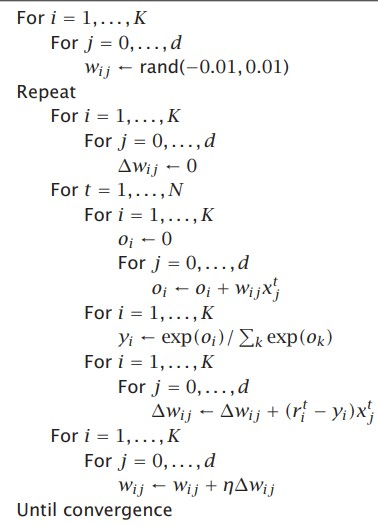
\includegraphics[width = 0.4\textwidth]{../images/logi_gradm.jpg}
\end{figure}


\newpage
\begin{lstlisting}[language=Python, caption=Logistic Regression Code]

class LogisticRegression():
  def __init__(self,w, learning_rate,num_epochs):
    self.w = w
    self.learning_rate = learning_rate
    self.num_epochs = num_epochs
   
  def sigmoid(self,x):
    return 1/(1 + np.exp(-x))

  def train(self,X, y):
    n, m = X.shape
    
    
    for epoch in range(self.num_epochs):
      y_hat = [self.sigmoid(w@X[i]) for i in range(n)]
      error = -(np.sum([y[i]*np.log(y_hat[i]) + (1-y[i])*np.log(1-y_hat[i]) for i in range(n)]))
      dw = X.T@(y-y_hat)
      self.w = self.w - self.learning_rate*dw
    return y_hat, error, self.w

  def predict(self,X, w):
    y_pred = self.sigmoid(X@w)
    y_class = [1 if i > 0.5 else 0 for i in y_pred]
    return y_class

  def accuracy(self,y_true, y_pred):
    return np.mean([1 if (y_true[i]==y_pred[i]) else 0 for i in range(len(y_pred))])


\end{lstlisting}

\subsection*{Questions}

\begin{questions}
\question[]Parameters of Logistic regression model are estimated using maximum likelihood estimation(MLE). State true or false.
\question[]Logit function gives \rule{2cm}{0.15mm}of output variable.
\question[] Does the probability sum equal to 1 for sigmoid function in Logistic regression?
\begin{choices}
\choice Yes, always.
\choice Not always.
\end{choices}
\question[] What can be done to avoid over-fitting in the model?
\question[] Which metric should be used to compare the logistic regression model output to the target variable?\\
\begin{oneparchoices}
\choice AUC-ROC curve
\choice Logloss
\choice MSE
\end{oneparchoices}
\end{questions}










\end{document}